%% 
%% Copyright 2019-2024 Elsevier Ltd
%% 
%% This file is part of the 'CAS Bundle'.
%% --------------------------------------
%% 
%% It may be distributed under the conditions of the LaTeX Project Public
%% License, either version 1.3c of this license or (at your option) any
%% later version.  The latest version of this license is in
%%    http://www.latex-project.org/lppl.txt
%% and version 1.3c or later is part of all distributions of LaTeX
%% version 1999/12/01 or later.
%% 
%% The list of all files belonging to the 'CAS Bundle' is
%% given in the file `manifest.txt'.
%% 
%% Template article for cas-sc document for 
%% double column output.

\documentclass[a4paper,fleqn]{cas-sc}
\usepackage{hyperref}
% If the frontmatter runs over more than one page
% use the longmktitle option.
%\documentclass[a4paper,fleqn,longmktitle]{cas-sc}

%\usepackage[numbers]{natbib}
%\usepackage[authoryear]{natbib}
\usepackage{float}
\usepackage[authoryear]{natbib}
\usepackage{csquotes}
\usepackage{algorithm2e}
\usepackage{placeins}
\usepackage{xcolor} 
\usepackage{capt-of}

%%%Author macros
\def\tsc#1{\csdef{#1}{\textsc{\lowercase{#1}}\xspace}}
\tsc{WGM}
\tsc{QE}
%%%

% Uncomment and use as needed
%\newtheorem{theorem}{Theorem}
%\newtheorem{lemma}[theorem]{Lemma}
%\newdefinition{rmk}{Remark}
%\newproof{pf}{Proof}
%\newproof{pot}{Proof of Theorem \ref{thm}}

\usepackage{xcolor}   % put this in your preamble

% helper macro
\newcommand{\red}[1]{\textcolor{black}{#1}}

\usepackage[many]{tcolorbox}
\usepackage{xcolor}
\usepackage{varwidth}
\usepackage{environ}
\usepackage{xparse}
\usepackage{makecell}
\usepackage{tabularx}


\begin{document}
\let\WriteBookmarks\relax
\def\floatpagepagefraction{1}
\def\textpagefraction{.001}

% Short title
\shorttitle{Explanations of LLM Biases}    
% Explaining LLM Biases Impacts Emotional and Analytical Trust Differently Between WEIRD and non-WEIRD Populations
\title [mode=title]{Explanations of LLM Biases Impact Emotional and Analytical Trust Differently Between WEIRD and NORMAL Individuals}

% Short author
\shortauthors{Malloy, Wax, Klein}  
\author[1]{Tailia Malloy*}[
            orcid=0000-0003-2512-984X
            ]
\ead{tailiamalloy@gmail.com}
\author[1]{Jules Wax*}[
            orcid=0000-0003-2512-984X
            ]
\ead{tailiamalloy@gmail.com}

\author[1]{Tegawende F. Bissyande}[
            orcid=0000-0003-2512-984X
            ]
\ead{tailiamalloy@gmail.com}

\author[1]{Jacques Klein}[
            orcid=0000-0003-2512-984X
            ]
\ead{tailiamalloy@gmail.com}

\affiliation[1]{organization={Interdisciplinary Centre for Security, Reliability and Trust (SnT), University of Luxembourg}, addressline={29, avenue J.F. Kennedy},  country={Luxembourg }}
\affiliation[]{*Co-first authors. corresponding author: Tailia Malloy.}


% Here goes the abstract
\begin{abstract}
Methods for improving human trust in Large Language Models (LLMs) have been extensively studied in recent research, with a focus on demonstrating improvement in trust through engagement with LLMs in contained experiment settings. Existing studies are limited in three ways, they seek to improve human trust in LLMs only, they have primarily focused on assessing analytical definitions of trust alone, and they have drawn from exclusively Western, Educated, Industrialized, and Democratic participant pools (WEIRD). As LLMs and AI systems that rely on them become more and more interconnected in our daily lives there is an increased relevance of the question of how humans form trust relationships differentially based on their demographics and the specific type of trust being assessed. In this work we present results from an online survey and an interactive LLM bias educational platform to differentiate between emotional and analytical trust with results from over 400 participants. Results show that interactive experiences demonstrating LLM biases decreases the emotional and analytical trust in LLMs for WEIRD participants, but increases emotional trust, while decreasing analytical trust, for NORMAL participants. Further analysis of participant open responses is explored to provide potential explanations for the differences between the impact of LLM behavioral explanations on trust. These results highlight the importance of multi-faced conceptualizations of trust relationships in Human-Computer Interaction research, and of understanding the similarities and differences between WEIRD and non-WEIRD populations in how they trust AI systems. 
\end{abstract}

\begin{keywords}
Human Computer Interaction, 
Trustworthy Artificial Intelligence, 
Large Language Models, 
\end{keywords}
\maketitle

\section{Introduction}
Currently the stock market capitalization of the top companies providing AI services and hardware in the United States of America (NVIDIA, Alphabet, Apple, Amazon, Meta, OpenAI, Anthropic) are collectively valued at over \$30 Trillion USD, approximately 30\% of the USA economy as measured by market capitalization and roughly 20\% of the net profits of the S\&P500 in 2025. These evaluations and profits are built on the fundamental necessity for individuals and organizations to place their trust in AI systems to be used as tools, sources of information, and increasingly as autonomous agents that make their own decisions while acting independently of human oversight. The societal impact of the trust that humans place in AI systems has had positive impacts in areas such as diagnostics and preventative medicine in healthcare \cite{}, transportation and logistics \cite{}, the quality, affordability, and access to education \cite{}, and the safety and security of online systems \cite{}. However, the goals of these private companies in increasing individual and institutional trust in these systems is becoming more and more divergent with the desired aims of users, with significant personal costs associated with placing too much trust in AI systems. One of the ways that the divergence of the goals of AI companies and end-users is most clear is in the differential impact that the introduction of these technologies has had and will have on the global south when compared to the western economies where these companies are centered. 

Significant effort from research institutions as well as monetary investment from private companies has gone towards the goal of increasing the trust that humans have in AI systems. This necessity is due to the significant biases that are inherent in LLMs due to being trained primarily to predict the next portion of a word in a sequence based on the statistical regularities of text generated by the entire history of human writing. This results in predictive models that are biased in the same ways that humans were biased in the past, particularly those who were affluent and important enough to have their words written down, and continue to be biased today. One of the major breakthroughs in improving the trust of AI systems in spite of these biases has been in the development of Reinforcement Learning from Human Feedback (RLHF) which trains LLMs with a so-called \textit{alignment} objective that seeks to increase the perceived quality of system responses. The data used to train these models initial involved workers, often in the global south, evaluating and ranking model output 

In line with the research and private company goals of increasing trust, many studies have been performed with human subjects that sought to demonstrate methods for increasing the level of trust that users have in these systems. A typical structure of this type of study is to have participants fill in a questionnaire to report their level of trust in AI systems, and then engage in either a passive reading, listening, or watching experience or an active interaction experience with an AI system, before repeating the same or a similar questionnaire \cite{}.  However, since the goals of private companies and researchers has typically been in increasing trust, little attention has been given into how descriptions of biases or limitations of AI can impact the trust users have in them. Additionally, the populations that these studies typically draw from primarily focus on easy to collect participants such as from universities, end-users, and personal circles, known commonly in the literature as WEIRD (Western, Educated, Industrialized, Rich, and Democratic). The effect of evaluating a primarily western population for improvements in trust while initially relying primarily on data annotated by workers in the global south is multiplicative, as the public perception of how AI is and should be trusted is conceived of through the lens of individuals who are separated from the human costs of AI training while also being disproportionately more likely to benefit from its proliferation. 

Research studying human trust has additionally relied on an analytical definition of trust, in line with western scientific ideals of logical and non-emotional explanations of behavior and psychology \cite{}. In contrast, western philosophical tradition and oral histories of the global south have often put significant or equal emphasis on an emotional understanding of behavior and justifications for actions. This has lead to an additional amplifying effect of how we conceive of the trust of AI systems, as it has eschewed focus on alternative conceptualizations of trust, psychology, and ethics. The potential effect of this over-focus and restrictive definition can be linked to the high prevalence of poor mental health outcomes for some users of popular AI systems \cite{}, which is frequently downplayed and said to be irrelevant by the companies that operate these systems \cite{}. Instead, these companies and institutions pressuring for expanded adoption of AI systems prefer a more purely utilitarian perspective of the assessment of AI success, by which the benefits in areas like reduced traffic deaths are seen as equally relevant and able to offset areas like the failure of AI systems used in war to make for more efficient operation of genocide \cite{} and mistakes resulting in the deaths of innocent children \cite{}. 

For the purposes of avoiding repeated usage of the term 'non-WEIRD', which defines the culture and unique experiences of those who do not fit into the WEIRD demographics in opposition to a group that has historically benefited from their subjugation, we will employ a novel acronym NORMAL to mean Native, Orally-educated, Relational, Multi-generational, Ancestral, and Local (NORMAL). This specific acronym is devised to highlight the particularly relevant features of these groups that can influence how they form trust relationships with other humans and how this impacts their trust of AI systems. The research presented in this work seeks to fill a significant gap in the literature of LLM trust to better understand how different dimensions of trust, analytical vs. emotional, impact populations differentially, WEIRD vs. NORMAL. In the following sections related works in evaluating the trust of LLMs is presented to demonstrate the current understanding of how humans form trust relationships with LLMs, and how different ways of interacting with LLMs impact different dimensions of trust. After this, our experiment methodology is presented before detailing the results of the analysis including qualitative analysis of open responses and behavior during interaction with LLMs, and quantitative analysis of changes in reported levels of trust. The discussion and conclusions sections conclude this paper with a broader picture connecting the results we present with the current state of AI in research and society. 

\section{Background}
\subsection{Biases in AI and LLMs}
\subsubsection{Racial Biases}
\cite{buolamwini2018gender} Stochastic parrots, can LLMs be too big \cite{bender2021dangers}. AI and Blackness, towards moving beyond bias and representation... \cite{dancy2021ai}. The forgotten margins of AI ethics... \cite{birhane2022forgotten}. 
\iffalse
\subsubsection{Gender Biases}
\subsubsection{Intersectional Biases}

\subsection{WEIRD vs. NORMAL Trust}
\subsubsection{NORMAL Trust}
\subsubsection{WEIRD Trust}
\subsubsection{Evaluations of Trust}


\subsection{Trustworthy AI}
\subsubsection{Cognitive Science of Trustworthy AI}
\subsubsection{Human Factors in Trustworthy AI}
\subsubsection{Measuring Human Trust in AI}
\fi 

\section{Methodology}
\subsection{Measures}
\subsection{Hypotheses}
\textbf{Hypothesis 1.} Comparisons of pre and post experiment questionnaires will demonstrate a significant difference in trust scores for overall trust as aggregate measures as well as emotional and analytical trust aggregate measures individually.
1.1 compare pre-post for aggregate trust to show significant difference
1.2 compare pre-post for analytical trust to show a significant difference.
1.3 compare pre-post for emotional trust to show a significant difference.
Make a plot with 3 subplots in this order: overall, analytical, emotional.

\textbf{Hypothesis 2.} Comparing the type of trust, WEIRD participants will demonstrate a significant decrease in both analytical and emotional trust in both conditions, with a significant difference between the two types of trust (i.e., emotional and analytical trust will both decrease and differ from each other in magnitude).
2.1 pre-post will be significant in overall trust when looking at just WEIRD participants.
2.2 pre-post will be significant in analytical trust when looking at just WEIRD participants.
2.3 pre-post will be significant in emotional trust when looking at just WEIRD participants.
2.4 compare analytical and emotional standardized change to show a significant difference as predicted by the hypothesis.
Make a plot with 4 subplots in this order: overall, analytical, emotional, emotional-vs-analytical difference.

\textbf{Hypothesis 3.} Comparing the type of trust, non-WEIRD participants will demonstrate a significant decrease in analytical and emotional trust in both conditions, with no significant difference between the magnitude of the two types of trust (i.e., emotional and analytical trust will both decrease with no significant difference between each other).
3.1 pre-post will be significant in overall trust when looking at just NORMAL participants.
3.2 pre-post will be significant in analytical trust when looking at just NORMAL participants.
3.3 pre-post will be significant in emotional trust when looking at just NORMAL participants.
3.4 compare analytical and emotional standardized change to show that there is no significant difference as predicted by the hypothesis.
Make a plot with 4 subplots in this order: overall, analytical, emotional, emotional-vs-analytical difference.

\textbf{Hypothesis 4.} Group and condition will show distinct effects across trust dimensions and these effects should be visualized in a three-panel grouped-bar figure.
4.1 analytical trust change by Group x Condition with paired pre-post significance markers within each cell.
4.2 emotional trust change by Group x Condition with paired pre-post significance markers within each cell.
4.3 analytical-vs-emotional change difference by Group x Condition with within-condition WEIRD vs NORMAL significance markers.
Recreate the three-panel Group x Condition design and color scheme (Interactive blue, Static/Text orange) with non-overlapping significance annotations.

\section{Results and Analysis}
\subsection{Hypothesis 1}
\begin{center}
\centering
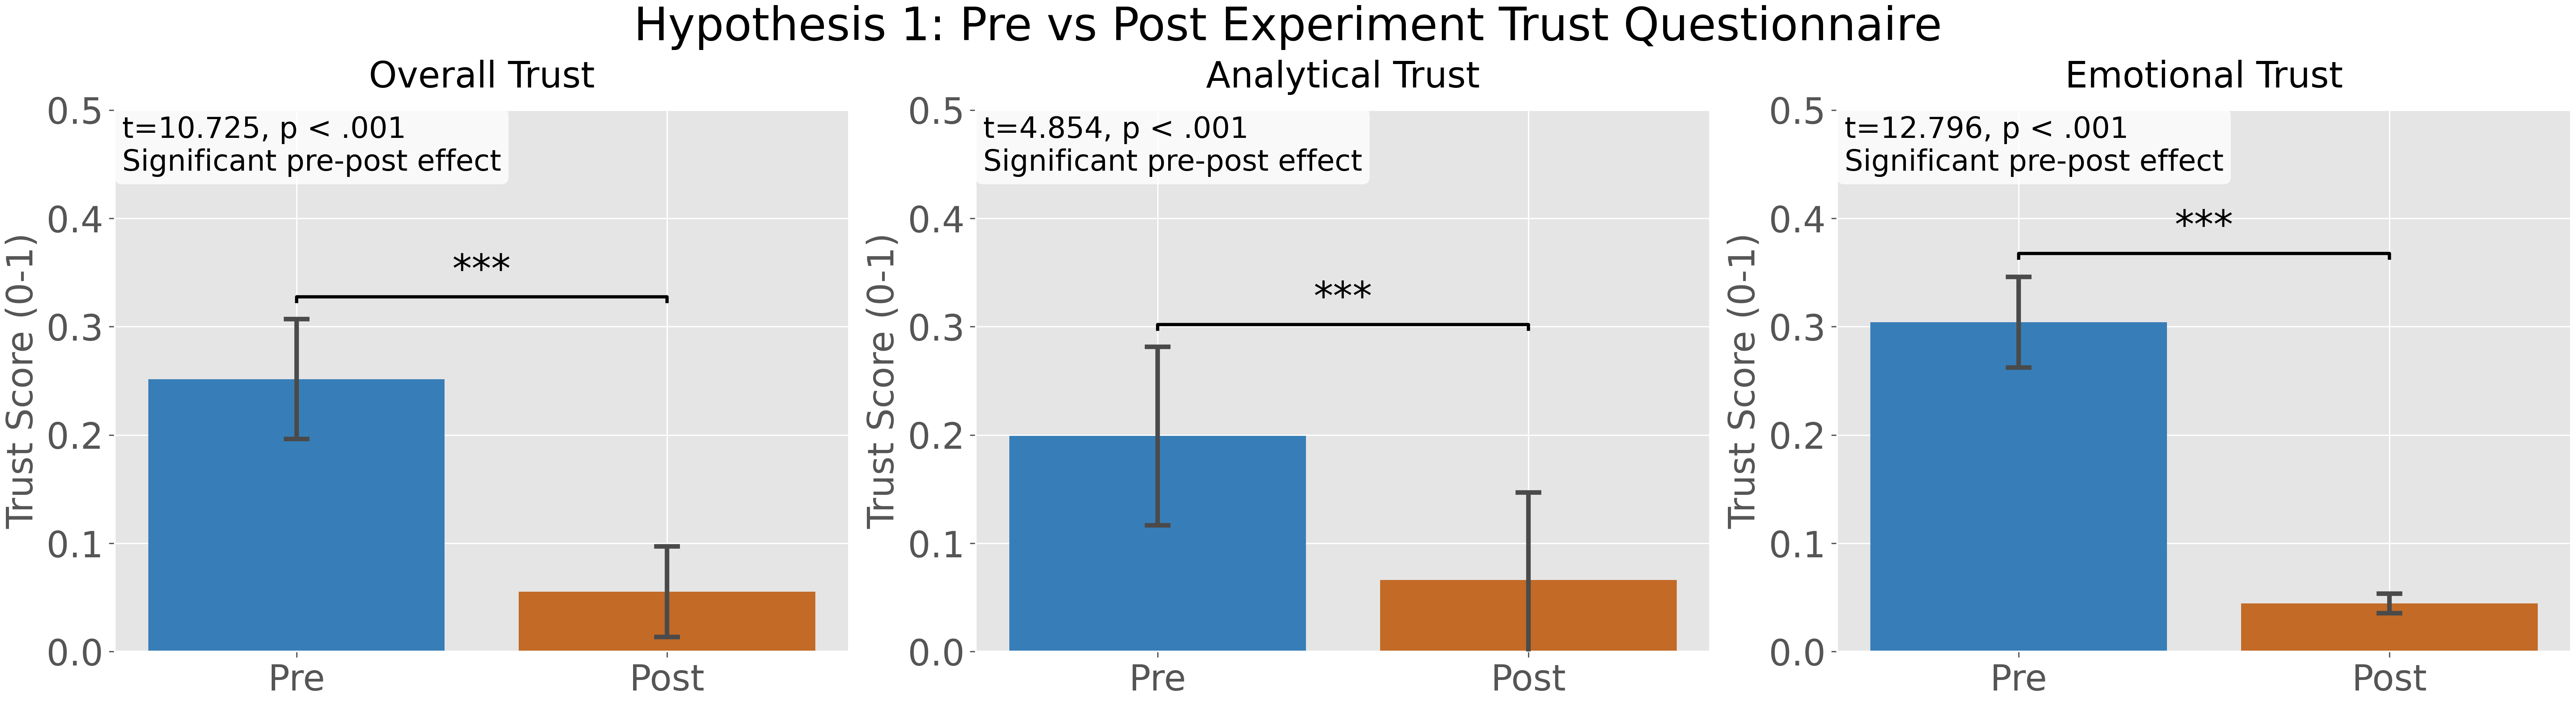
\includegraphics[width=0.85\linewidth]{Figures/hypothesis1.png}
\captionof{figure}{Visualization for Hypothesis 1.}
\label{fig:hypothesis1}
\end{center}

To begin our statistical analysis with Hypothesis 1, we perform a comparison of the pre and post experiment questionnaires in terms of overall, analytical alone, and emotional alone self-reported trust. This results in three sub-hypotheses related to this hypothesis that can each be individually tested for statistical significance. 

Hypothesis 1.1 compares the pre-post experiment overall trust, to evaluate the significance in the change in reported trust when combining emotional and analytical definitions. We performed a two-tailed paired-samples t-test ($\alpha=.05$) and a two-sided Wilcoxon signed-rank test on pre-post overall trust scores, which showed $n=504$, $M_{pre}=4.728$, $SD_{pre}=12.319$, $M_{post}=1.062$, $SD_{post}=9.561$, $t(503)=10.395$, $p < .001$, $W=27993.500$, $p_{W} < .001$, $d=-0.463$, $\Delta=-3.667$, sub-hypothesis supported. Hypothesis 1.2 compares the pre-post experiment analytical trust, to evaluate the significance in the change in reported analytical trust. We performed the same two-tailed paired-samples t-test and two-sided Wilcoxon signed-rank test on pre-post analytical trust scores, which showed $n=504$, $M_{pre}=1.990$, $SD_{pre}=9.439$, $M_{post}=0.661$, $SD_{post}=9.238$, $t(503)=4.854$, $p < .001$, $W=35605.500$, $p_{W} < .001$, $d=-0.216$, $\Delta=-1.329$, sub-hypothesis supported. Hypothesis 1.3 compares the pre-post experiment emotional trust, to evaluate the significance in the change in reported emotional trust. We performed the same two-tailed paired-samples t-test and two-sided Wilcoxon signed-rank test on pre-post emotional trust scores, which showed $n=504$, $M_{pre}=2.738$, $SD_{pre}=4.309$, $M_{post}=0.401$, $SD_{post}=0.917$, $t(503)=12.796$, $p < .001$, $W=15999.000$, $p_{W} < .001$, $d=-0.570$, $\Delta=-2.337$, sub-hypothesis supported.

These results demonstrate that there is a significant change in the reported trust when averaging over each condition (Interactive vs. Text), type of trust (Emotional vs. Analytical), and demographic groups (WEIRD vs. NORMAL). This provides the necessary statistical foundation supporting our first hypothesis. Additionally, this overall difference supports the structuring of the following statistical tests used to evaluate the subsequent hypotheses. 

\subsection{Hypothesis 2}
\begin{center}
\centering
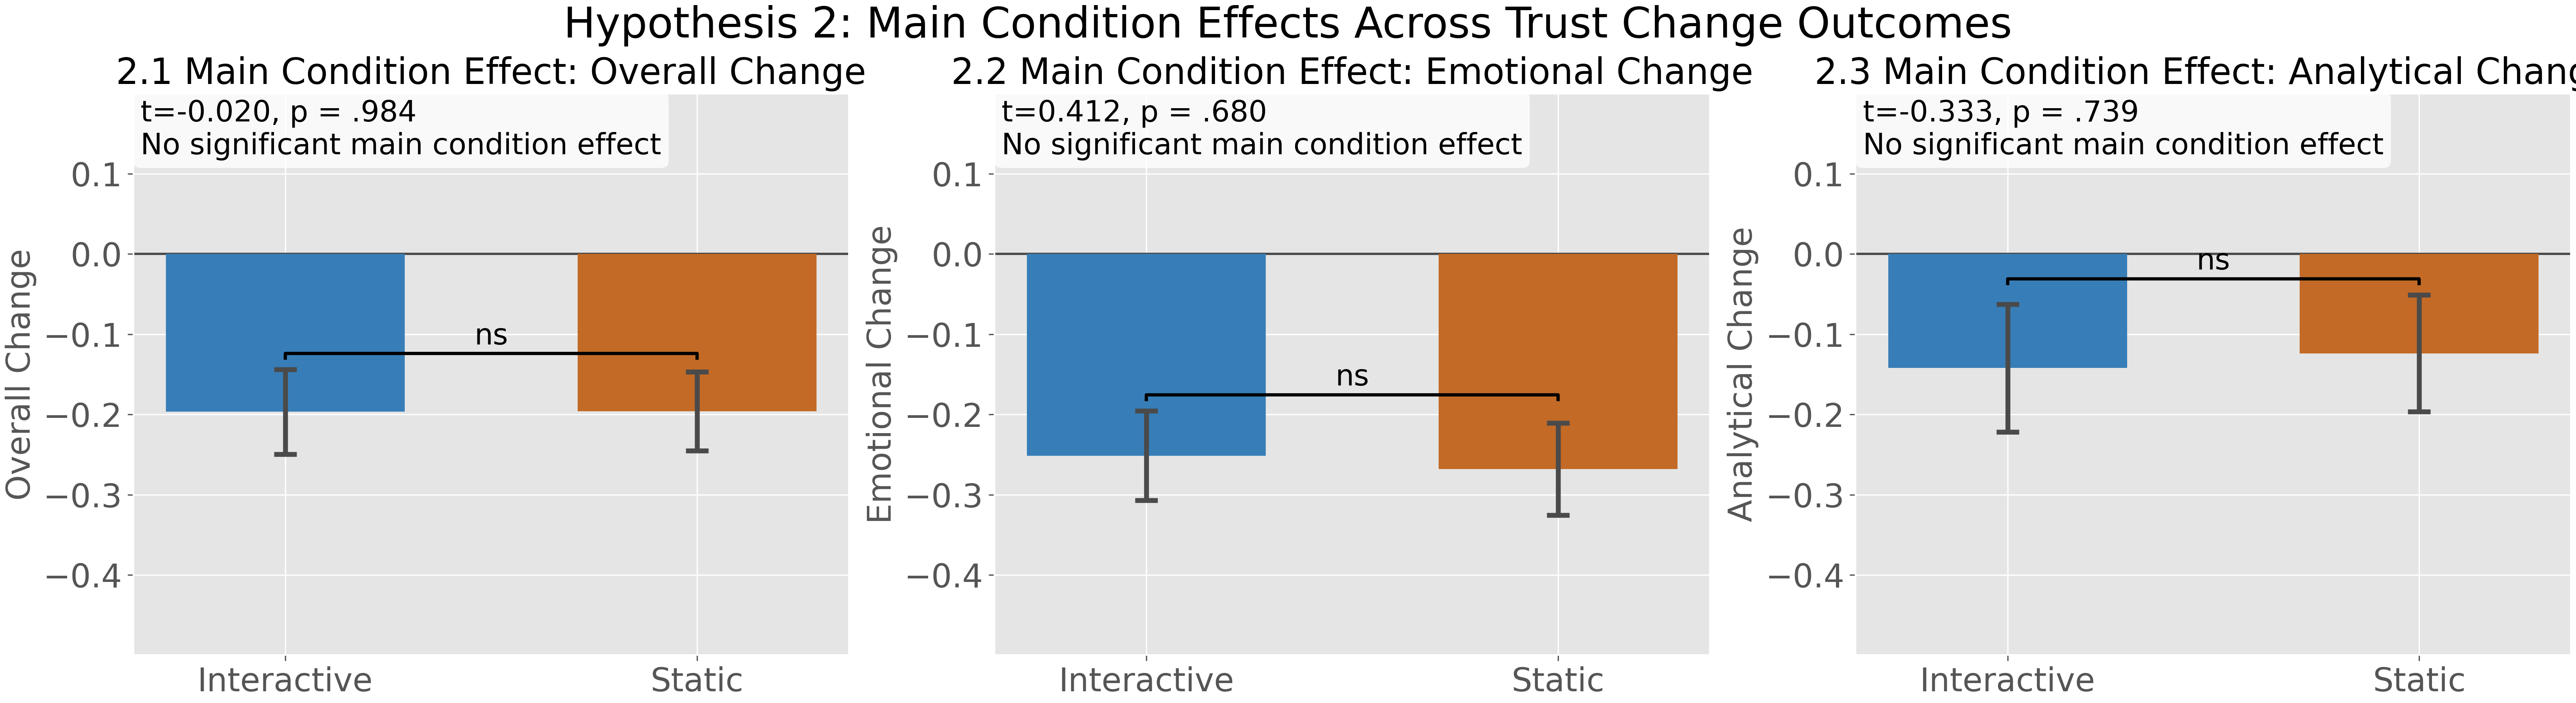
\includegraphics[width=0.85\linewidth]{Figures/hypothesis2.png}
\captionof{figure}{Visualization for Hypothesis 2.}
\label{fig:hypothesis2}
\end{center}

For Hypothesis 2, we evaluate WEIRD participants only and test whether overall, analytical, and emotional trust all decrease from pre to post, and whether the standardized emotional-versus-analytical change differs in magnitude. This produces four sub-hypotheses that are each evaluated with inferential statistics.

Hypothesis 2.1 compares pre-post overall trust within WEIRD participants. We performed a two-tailed paired-samples t-test ($\alpha=.05$) and a two-sided Wilcoxon signed-rank test, which showed $n=120$, $M_{pre}=1.217$, $M_{post}=-1.133$, $t(119)=3.440$, $p < .001$, $W=1848.000$, $p_{W} < .001$, $d=-0.314$, $\Delta=-2.350$, sub-hypothesis supported. Hypothesis 2.2 compares pre-post analytical trust within WEIRD participants. We performed the same two-tailed paired-samples t-test and two-sided Wilcoxon signed-rank test, which showed $n=120$, $M_{pre}=-0.167$, $M_{post}=-1.683$, $t(119)=3.014$, $p = .003$, $W=1624.500$, $p_{W} = .003$, $d=-0.275$, $\Delta=-1.517$, sub-hypothesis supported. Hypothesis 2.3 compares pre-post emotional trust within WEIRD participants. We performed the same two-tailed paired-samples t-test and two-sided Wilcoxon signed-rank test, which showed $n=120$, $M_{pre}=1.383$, $M_{post}=0.550$, $t(119)=2.058$, $p = .042$, $W=1936.000$, $p_{W} = .041$, $d=-0.188$, $\Delta=-0.833$, sub-hypothesis supported. Hypothesis 2.4 compares standardized emotional and analytical change within WEIRD participants. We performed a paired comparison using a two-tailed paired-samples t-test and a two-sided Wilcoxon signed-rank test, which showed $n=120$, $M_{em,z}=0.367$, $M_{an,z}=-0.030$, $t(119)=3.301$, $p = .001$, $W=2436.000$, $p_{W} = .002$, $d=0.301$, $\Delta_{z}=0.398$, sub-hypothesis supported.

These results indicate that WEIRD participants show significant decreases across all three trust aggregates and a significant emotional-versus-analytical standardized difference, supporting Hypothesis 2.

\subsection{Hypothesis 3}
\begin{center}
\centering
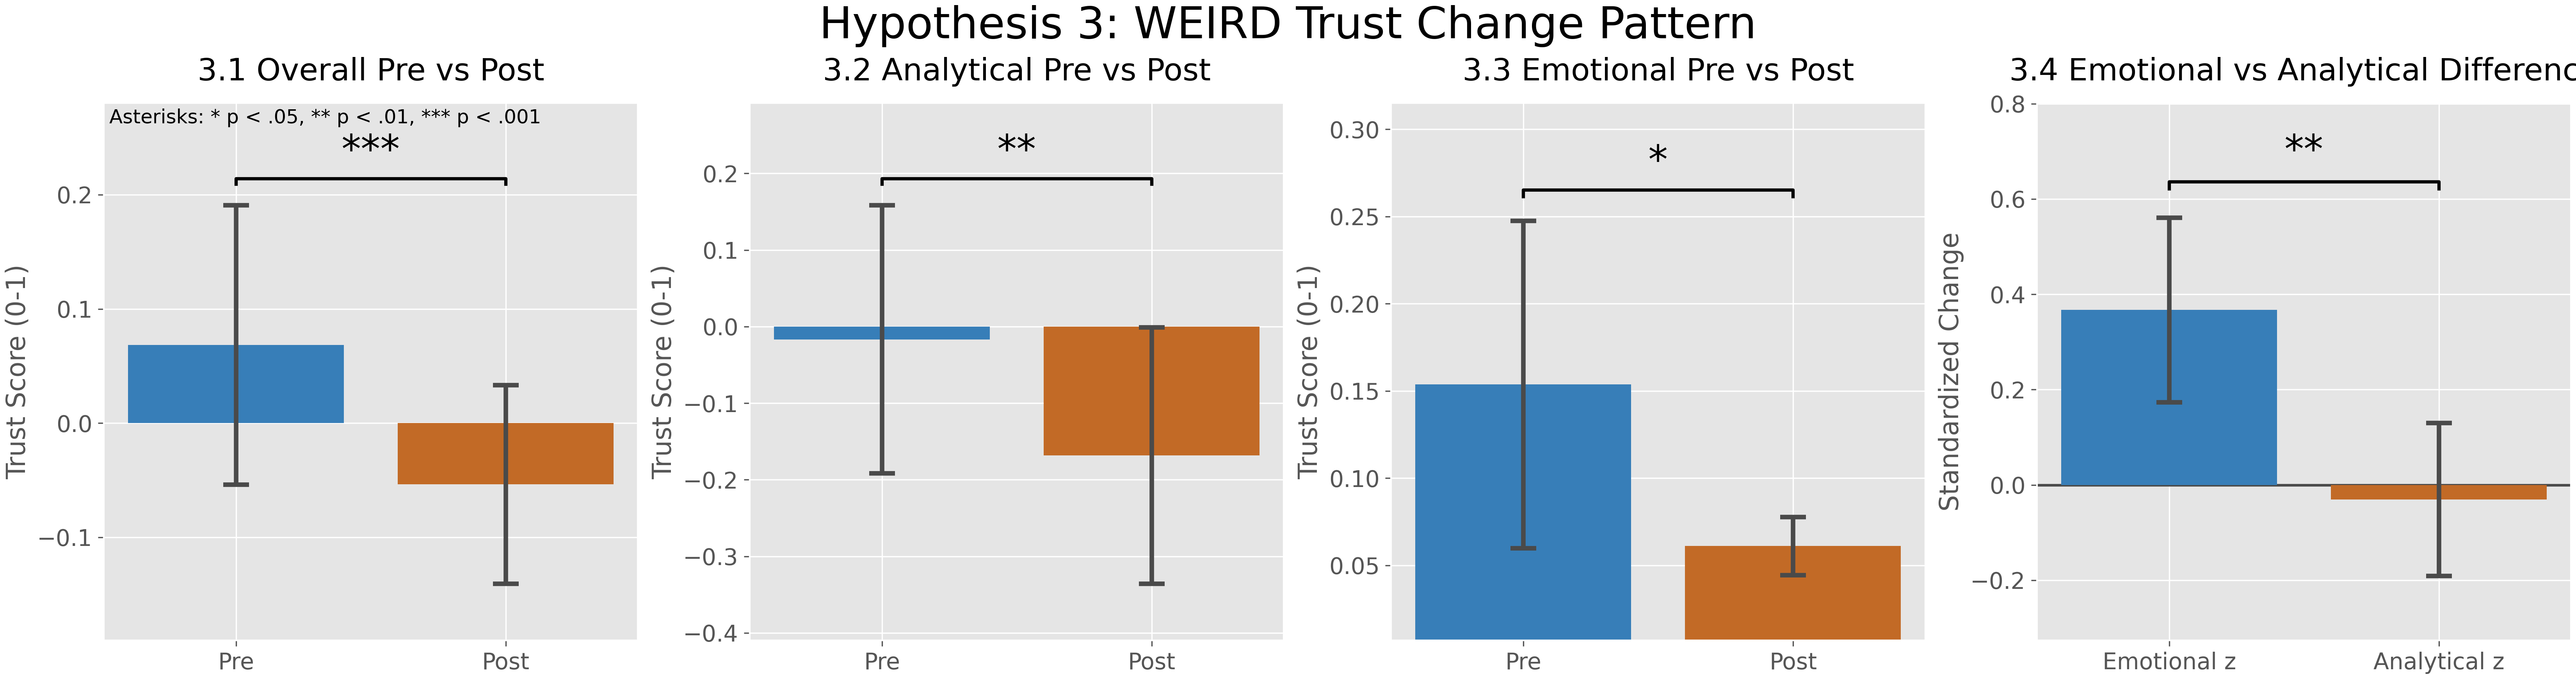
\includegraphics[width=0.85\linewidth]{Figures/hypothesis3.png}
\captionof{figure}{Visualization for Hypothesis 3.}
\label{fig:hypothesis3}
\end{center}

For Hypothesis 3, we evaluate NORMAL (non-WEIRD) participants and test whether overall, analytical, and emotional trust decrease from pre to post, while expecting no strong difference between standardized emotional and analytical change.

Hypothesis 3.1 compares pre-post overall trust within NORMAL participants. We performed a two-tailed paired-samples t-test ($\alpha=.05$) and a two-sided Wilcoxon signed-rank test, which showed $n=384$, $M_{pre}=5.826$, $M_{post}=1.747$, $t(383)=9.970$, $p < .001$, $W=15536.500$, $p_{W} < .001$, $d=-0.509$, $\Delta=-4.078$, sub-hypothesis supported. Hypothesis 3.2 compares pre-post analytical trust within NORMAL participants. We performed the same two-tailed paired-samples t-test and two-sided Wilcoxon signed-rank test, which showed $n=384$, $M_{pre}=2.664$, $M_{post}=1.393$, $t(383)=3.928$, $p < .001$, $W=21912.000$, $p_{W} = .002$, $d=-0.200$, $\Delta=-1.271$, sub-hypothesis supported. Hypothesis 3.3 compares pre-post emotional trust within NORMAL participants. We performed the same two-tailed paired-samples t-test and two-sided Wilcoxon signed-rank test, which showed $n=384$, $M_{pre}=3.161$, $M_{post}=0.354$, $t(383)=14.183$, $p < .001$, $W=6354.500$, $p_{W} < .001$, $d=-0.724$, $\Delta=-2.807$, sub-hypothesis supported. Hypothesis 3.4 compares standardized emotional and analytical change within NORMAL participants. We performed a paired comparison using a two-tailed paired-samples t-test and a two-sided Wilcoxon signed-rank test, which showed $n=384$, $M_{em,z}=-0.115$, $M_{an,z}=0.010$, $t(383)=-1.923$, $p = .055$, $W=32037.000$, $p_{W} = .024$, $d=-0.098$, $\Delta_{z}=-0.124$.

These results show strong pre-post trust decreases in NORMAL participants across overall, analytical, and emotional trust. For the emotional-versus-analytical standardized contrast, the t-test is non-significant while Wilcoxon is significant, indicating mixed but small-magnitude evidence relative to the hypothesis expectation.

\subsection{Hypothesis 4}
\begin{center}
\centering
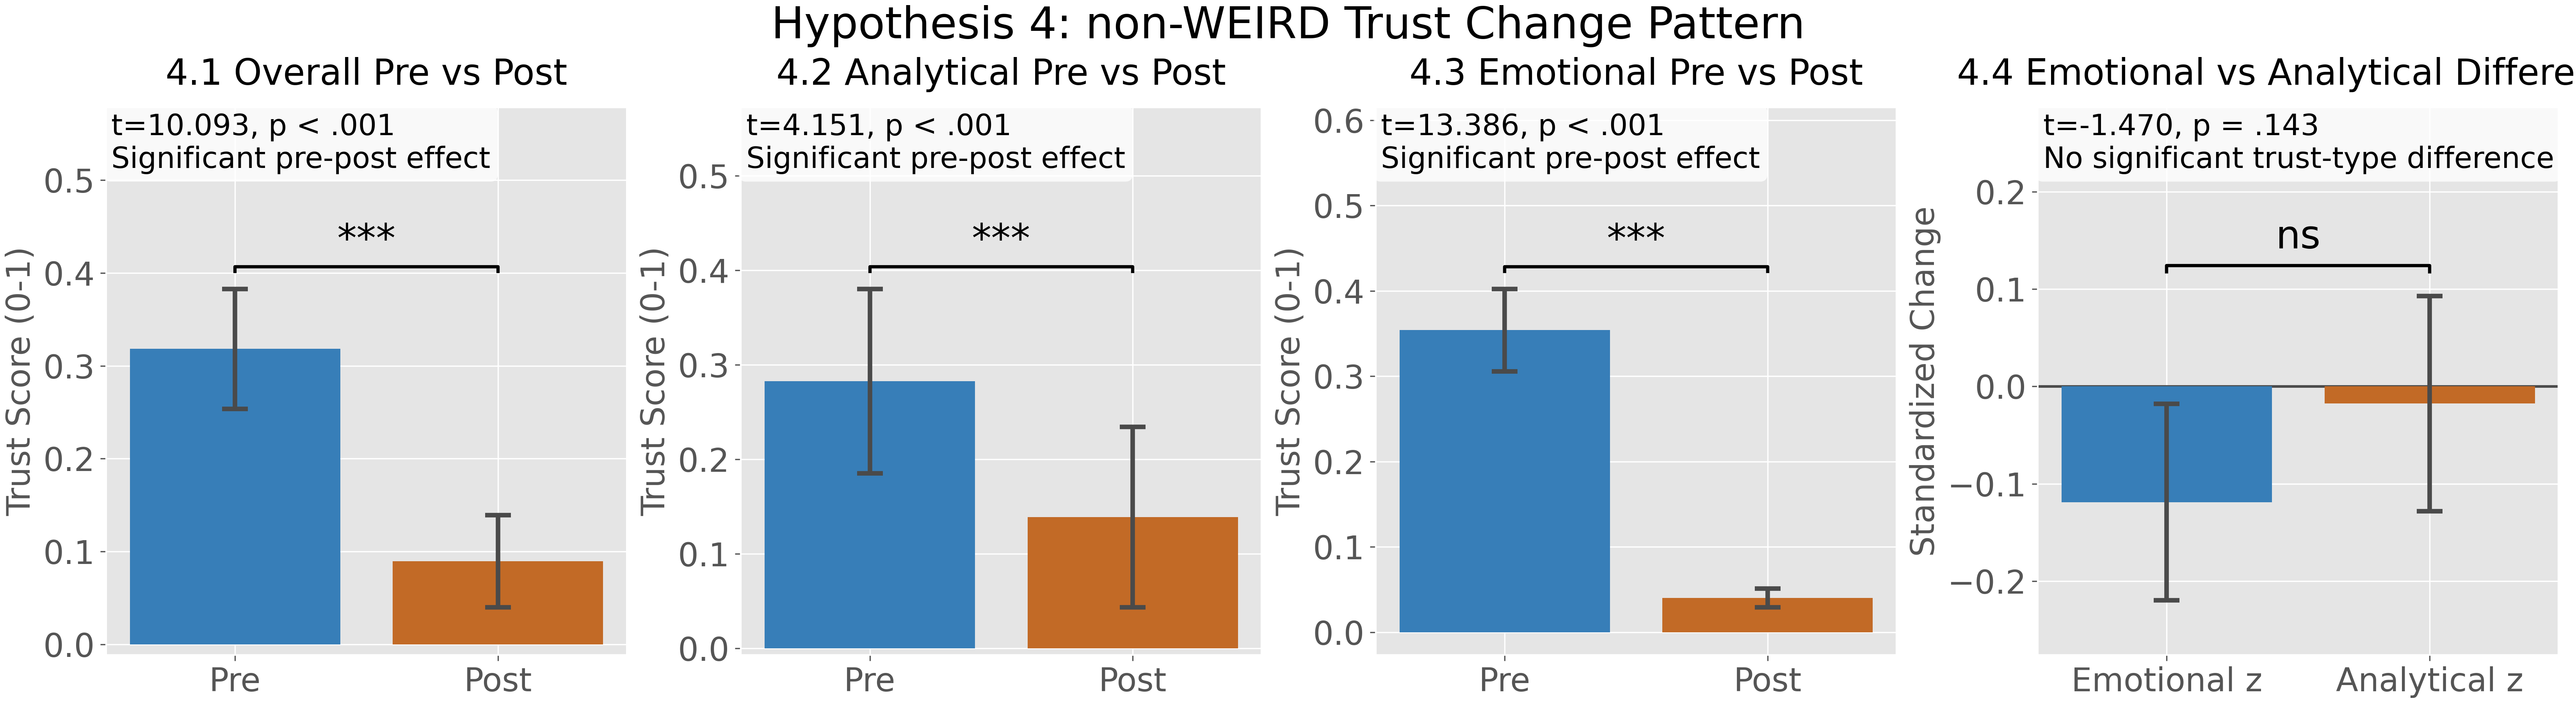
\includegraphics[width=0.85\linewidth]{Figures/hypothesis4.png}
\captionof{figure}{Visualization for Hypothesis 4.}
\label{fig:hypothesis4}
\end{center}

For Hypothesis 4, we test Group $\times$ Condition effects across analytical trust change, emotional trust change, and the analytical-versus-emotional difference metric in a three-panel design. All trust-change outcomes are computed as average change scores (Post - Pre).

Hypothesis 4.1 evaluates analytical trust change by Group $\times$ Condition. We performed within-cell pre-post paired-samples t-tests, plus an omnibus four-cell ANOVA and an OLS interaction estimate. Paired results were WEIRD/Interactive: $t(59)=2.17$, $p = .034$, $\Delta M=-0.180$; WEIRD/Static (Text): $t(59)=2.14$, $p = .037$, $\Delta M=-0.123$; NORMAL/Interactive: $t(191)=2.81$, $p = .006$, $\Delta M=-0.130$; NORMAL/Static (Text): $t(191)=2.74$, $p = .007$, $\Delta M=-0.124$. Omnibus ANOVA: $F=0.14$, $p = .938$. Interaction estimate: $b=-0.050$, $t(500)=-0.39$, $p = .696$. Hypothesis 4.2 evaluates emotional trust change by Group $\times$ Condition with the same test structure. Paired results were WEIRD/Interactive: $t(59)=1.71$, $p = .092$, $\Delta M=-0.104$; WEIRD/Static (Text): $t(59)=1.22$, $p = .229$, $\Delta M=-0.081$; NORMAL/Interactive: $t(191)=9.48$, $p < .001$, $\Delta M=-0.297$; NORMAL/Static (Text): $t(191)=10.57$, $p < .001$, $\Delta M=-0.326$. Omnibus ANOVA: $F=7.49$, $p < .001$. Interaction estimate: $b=-0.051$, $t(500)=-0.55$, $p = .585$. Hypothesis 4.3 evaluates analytical-vs-emotional change difference by Group $\times$ Condition. We performed Welch independent-samples tests within each condition, plus an omnibus four-cell ANOVA and an OLS interaction estimate. Condition-level Welch results were Interactive: $t=-2.28$, $p = .025$, $M_{WEIRD}=-0.076$, $M_{NORMAL}=0.167$; Static (Text): $t=-2.46$, $p = .015$, $M_{WEIRD}=-0.042$, $M_{NORMAL}=0.202$. Omnibus ANOVA: $F=3.82$, $p = .010$. Interaction estimate: $b=0.001$, $t(500)=0.01$, $p = .996$.

Overall, Hypothesis 4 shows meaningful main-pattern differences and significant within-condition group differences for the analytical-vs-emotional metric, but no reliable Group $\times$ Condition interaction in the regression interaction terms.

\subsection{Exploratory Qualitative Analysis Results}
\begin{center}
\centering
\includegraphics[width=0.9\linewidth]{Figures/sentiment.png}
\captionof{figure}{Open-response sentiment by group and condition.}
\label{fig:exploratory_sentiment_group_condition}
\end{center}

\begin{center}
\centering
\includegraphics[width=0.92\linewidth]{Figures/sentiment_change.png}
\captionof{figure}{Sentiment versus trust-change outcomes.}
\label{fig:exploratory_sentiment_trust_changes}
\end{center}

To complement the quantitative hypothesis tests, we performed an exploratory qualitative sentiment analysis on open-response text fields (AI Interaction Feeling, AI Definition Feeling, Explanation Comment). We analyzed $n=504$ participants and tested whether sentiment differs by condition and WEIRD/NORMAL grouping and whether sentiment is associated with trust-change outcomes.

For sentiment level differences (group/condition), we performed Welch two-sample tests for condition contrasts and group contrasts and fit an OLS interaction model (Condition $\times$ Group). The overall condition contrast was non-significant ($p = .979$), the overall group contrast was non-significant ($p = .213$), and the interaction term was non-significant ($p = .881$). For sentiment-to-trust associations, we performed Pearson and Spearman correlations in the full sample, with follow-up Pearson tests in condition and group subsets when primary effects were significant. In the primary full-sample tests, overall trust change was non-significant ($p = .414$), analytical trust change was significant ($p = .006$), emotional trust change was significant ($p = .011$), and analytical-minus-emotional trust change was highly significant ($p < .001$). Across the full exploratory module, we ran 28 primary tests (7 significant) and 16 follow-up tests (8 significant).

These exploratory results suggest that sentiment itself did not differ globally by condition or WEIRD grouping, but sentiment variation was meaningfully related to analytical, emotional, and especially analytical-minus-emotional trust change. Because these analyses were exploratory, they should be interpreted as hypothesis-generating evidence for targeted confirmatory models.


\section{Conclusions}

\section{Discussion}

%% Loading bibliography style file
\end{document}

